\chapter{General State of the Art}


\section{Context}

To replace materials that are very practical but very problematic for our environment, convince people of the usefulness of the replacement. on the one hand, by making functional objects. But also by opening the door to new imaginations that broaden the scope of what's possible. that's why, in the same way as classical research, design helps to shape this problem. 
\begin{figure}[h] % Adjust the vertical placement
    \centering
    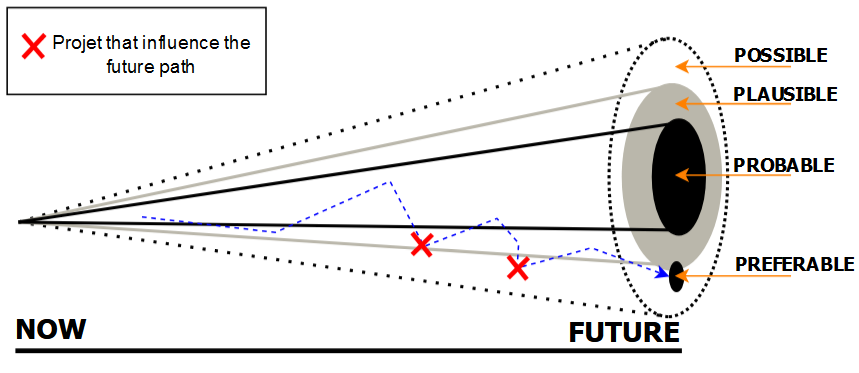
\includegraphics{images/futures_cone2.png}
    \caption{futures cone representation}
    \label{fig:futures code}
\end{figure}
Science in this field relatively new. The starting point differs depending on how define biomaterials and how make, or rather grow them. 
More globally, biomaterials are at the crossroads of many fields of scientific and even artistic research. From agriculture to design, from synthetic biology to fashion, from DIY fermented drink to biohacking in the kintchen\cite{CiteTheOdin}.
This is in line with new interdisciplinary courses integrating biodesign, such as MIT's "How To Grow (Almost) Anything" course\cite{CiteMITHTGAA}. 

As matter of fact, the starting point might be the first crops domestication. At this time the goal was only to produce food, and the process were optimized by selective breeding. By taking the plants with the biggest fruit or the best resistance to environment, from generation to generation plants were "optimized" for the population.
Besides, the use of wood are very use in numerous sectors\cite{ramage2017wood} push by international directive of less CO2 emmission and waste. 
  
However, today, biomaterials or biobased materials in this study are more in line with the aim of replace existing materials like plastics.
This biomaterials production projects are aimed to create in the futures of cone plausible or possible futures. 
Moreover the development of this new materials go hand in hand with the evolution of new machines for biomaterials. Bioreactors are controlled environment systems. There is no notable differences in hardware part from bioreactors in the litterature. The general form is a isolated space from outside environmental conditions, 
combine with a microcontroller responsible of sensors and actuator (i.e :fogger, fan, thermal resistance...). The microcontroller is also responsible to send data when monitoring is wanted. All powered by energy from different sources. 

Multiple reviews\cite{cottet2020biobased}\cite{vinod2020renewable}\cite{hairon2022bio} about biobased materials support for the fact that today's synthetic materials, especially those derived from oil, are a problem for human and ecosystem health.
These studies reveals the strong interess of these materials in term of sustainability and low cost production, and "by reducing wastages, landfills
and toxic emissions leading to greener and cleaner environment". They also show end proprieties these materials are distinguished by their biodegradability and compostability. Which also makes them interesting for their end-of-life properties. 
However, there are concers about a lack of large scale industrialisation and a lack standadise methodology \cite{andrew2022sustainable}. This leads to a lack of confidence in mechanical properties, as the absence of standardization, give rise to the limited exploitation of technical data on characteristics such as tensile strength, compression, fatigue, impact resistance and flammability, makes assessment more difficult.   
Into the bargain, most of these materials are and highly anisotropic.

\paragraph[short]{Industry} 
Ecovative and MycoWorks lead in mycelium-based biomaterials. Ecovative creates eco-friendly alternatives to plastics for packaging and construction, while MycoWorks focuses on sustainable mycelium leather, targeting fashion and luxury markets.
\paragraph[short]{In Design} 
Suzanne Lee, through Biofabricate, pioneers biofabrication in design, using biological processes to grow sustainable materials like microbial leather, pushing the boundaries of traditional manufacturing and eco-conscious design.


\section{Biomaterial}

The term biomaterials is used in many fields and doesn't quite describe the same thing. In the medical field, the term refers more to materials that are in contact (usually internal) with the human body without causing any harm. Here, the term biomaterials is used mainly to refer to materials produced by organisms, even though both functions are possible.

For the annual summit Biofabicate biomaterials correspond to several families of materials : 
biobased, Biofabicated, Bioassembled, Biosynthetic material. 

S.C.O.B.Y Lether and Mycelium-based material should be more in the Biofabicated definition. 

\begin{figure}[h] 
    \centering
    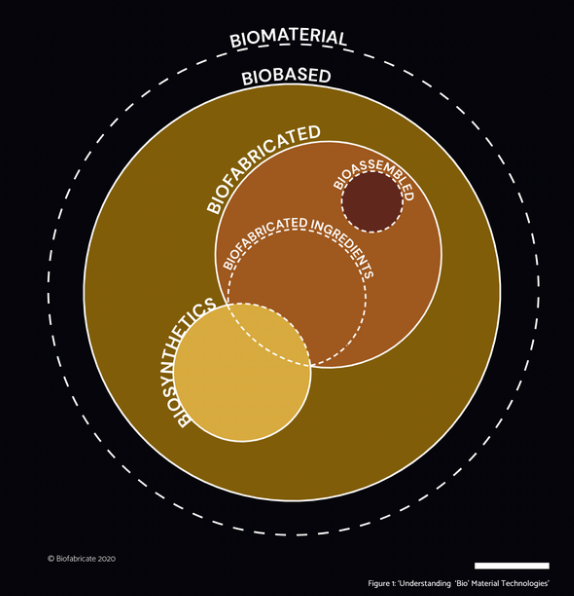
\includegraphics{images/defcircle.png}
    \caption{Bacterial definition circle}
    \label{fig:defcircle}
\end{figure}

\subsection{S.C.O.B.Y Lether} 

\begin{marginfigure}
    \centering
    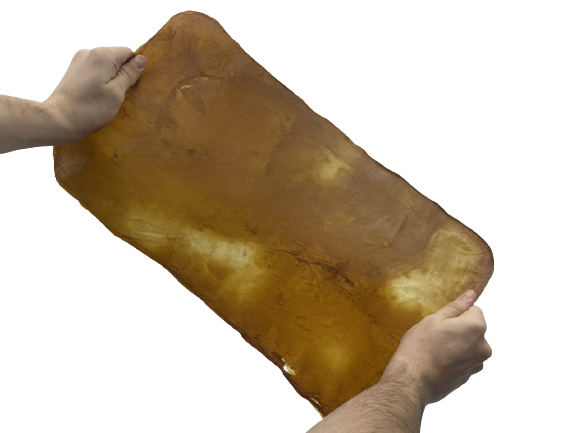
\includegraphics{images/kombucha-removebg-preview-removebg-preview.png}    
    \caption{S.C.O.B.Y Lether}
    \label{fig:S.C.O.B.Y Lether}
\end{marginfigure}

\paragraph[short]{Definition } 
S.C.O.B.Y, aim to Symbiotic Culture Of Bacteria and Yeast, during this symbiotic culture a lot of biochimical element are tranformed or exchanged by bacteria and yeast.
Among this biochimical elements, there is bacterial cellulose. Bacterial cellulose (BC) is a biopolymer that grows on the surface of the culture medium. which, once dry, produces a biomaterial with the appearance of leather. 

\begin{marginfigure}
    \centering
    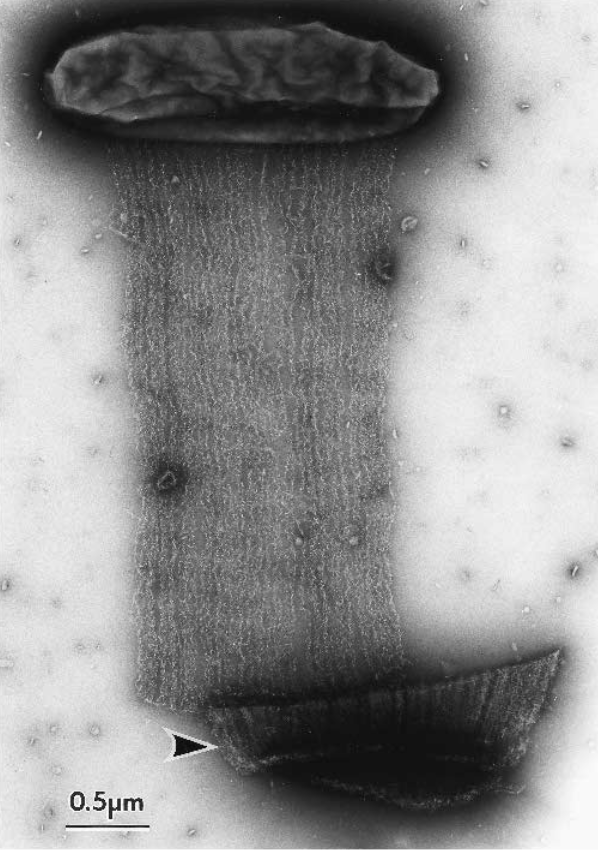
\includegraphics{images/bacteriaandcellulose.png}
    \caption{Negatively stained coarse band-like cellulose assembly produced during 6 h of incubation at 4 °C. At the bottom of the figure, a
    detached dense assembly of cellulose is also observed (indicated by the arrowhead)from\cite{hirai2002tem}}
    \label{fig:bacteriaandcellulose}
\end{marginfigure}

More precisely, 2 metabolic processes are at play, in a kind of “double” fermentation. 
on the one hand, alcoholic fermentation by yeasts. In other words, the glucoses will be converted into ehtanol. 
On the other hand, “acetic fermentation” by bacteria. In other words, the ethanol will be converted into acetic acid. see \ref{fig:fermentation formula} and \ref{fig:metabolic}

% C_6H_{12}O_6 + 2 \, \text{ADP} + 2 \, P_i \rightarrow 2 \, \text{ATP} + 2 \, H_2O + 2 \, \textcolor{red}{CH_3CH_2OH} + 2 \, CO_2

% \textcolor{red}{CH_3CH_2OH} + O_2 \rightarrow CH_3COOH + H_2O
\begin{figure}[h]
    \centering
    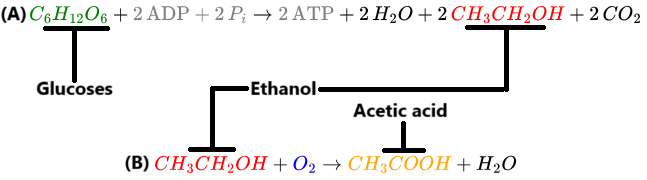
\includegraphics{images/formule-chimique.png}
    \caption{fermentation formulas, (A) : Alcoholic fermentation, (B) : Acetic fermentation}
    \label{fig:fermentation formula}
\end{figure}

\begin{figure}[h]
    \centering
    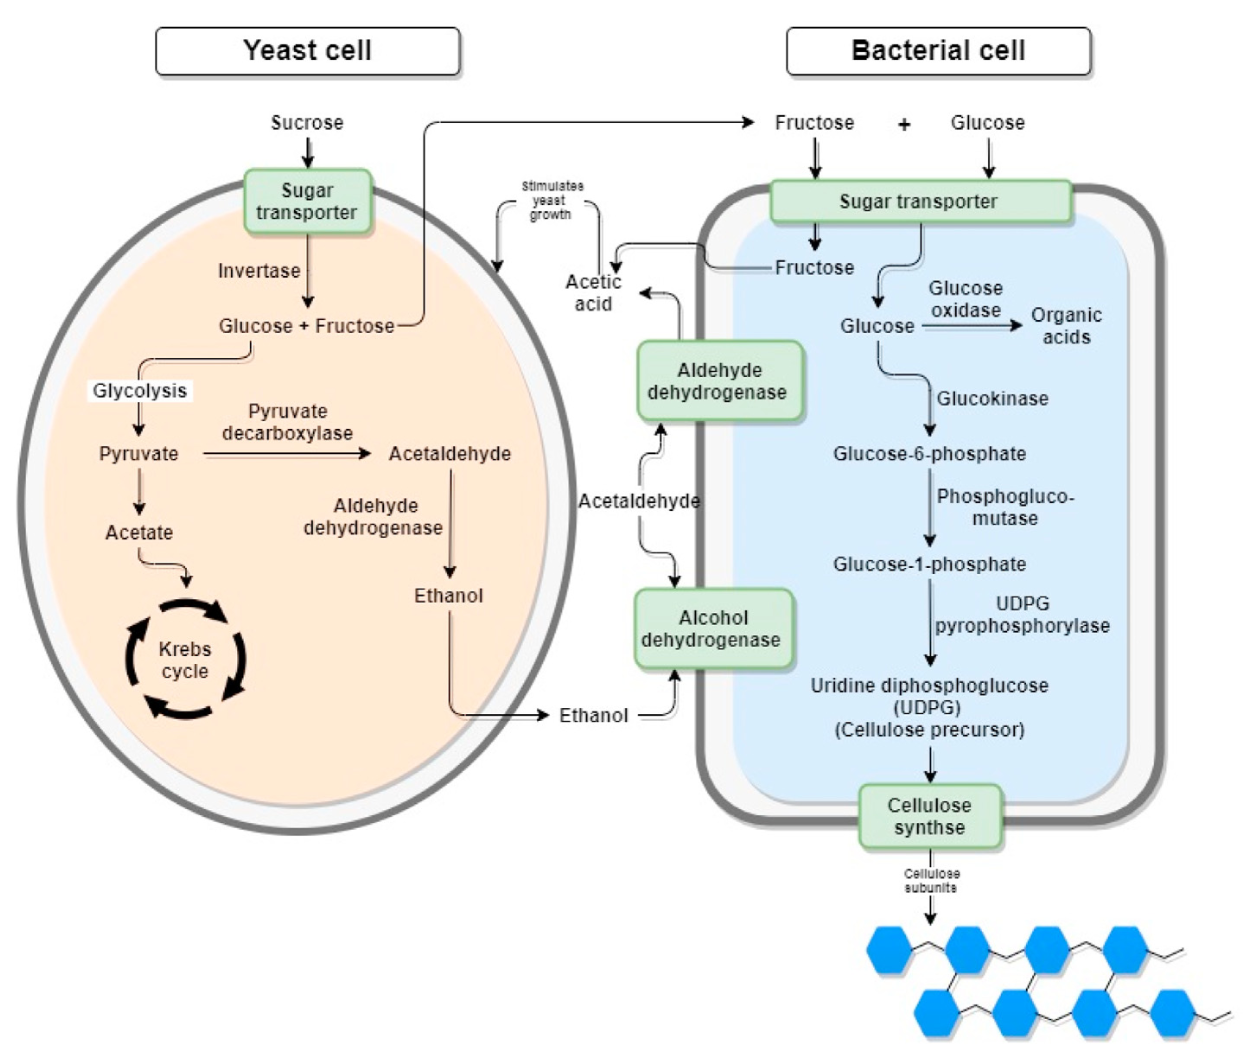
\includegraphics{images/schema_metabolique.png}
    \caption{Metabolism of substrates by the symbiotic culture of bacteria and yeast from\cite{laavanya2021current}}
    \label{fig:metabolic}
\end{figure}

In addition to the metabolic processes that allow these microorganisms to survive and reproduce, bacteria will also synthesize this so-called bacterial cellulose.\ref{fig:bacteriaandcellulose} 
More popularly, scoby is the culture used to make fermented tea-based drinks called kombucha. 
To grow cellulose, the recipe is similar: a strain of scoby, water, sugar and vinegar. The difference is that it is preferable first to select the strains that produce the most cellulose. 

Another element that emerges from the literature, without taking bioreactors into account, is that cellulose production decreases more and more over time and follows a kind of inverse exponential curve tending towards a finite value that corresponds to the maximum value of cellulose produced.\cite{chong2024modelling}.
as pictured \ref{biomasse-cellulose-grap}. There are two reasons why cellulose production stops: firstly, of course, because there is less and less nutrient in the culture medium; secondly, because the production of cellulose on the surface will eventually self-isolate the culture medium; and thirdly, as seen in equation (B) in \ref{fig:fermentation formula}, oxygen is important for bacterial fermentation, and therefore for their survival and development. 
\begin{marginfigure}
    \centering
    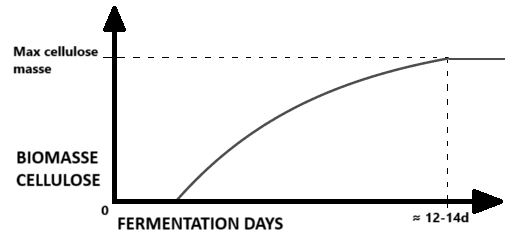
\includegraphics{images/biomasse-cellulose.png}
    \caption{model curve for cellulose biomasse over time}
    \label{fig:biomasse-cellulose-graph}
\end{marginfigure}

so, to sum up, in order to have good cellulose production, you need to maintain fermentation for the proper development of bacteria and yeast. at the same time, you need to make sure that the medium doesn't auto-asphyxiate.



\paragraph[short]{Use}

Roussel et al.'s extensive mapping\cite{roussel2023processes} effectively illustrates the diverse ecosystem around SCOBY leather production, showing Bacterial Cellulose (BC) is divided across varied fields: biology, medicine, food, textiles, and materials science. This broad range of applications reveals substantial potential, though these fields are rarely interconnected and often operate independently.
even if some of these applications are speculative or artistic, they tell us how a discipline approaches the problem of growth, and what the advantages and disadvantages of a particular approach are. Furthermore, it's interesting to note that a combined approach could give rise to projects with a strong impact on their dicipline. for example, between the industrial and medical machine clusters. 
\begin{figure}
    \centering
    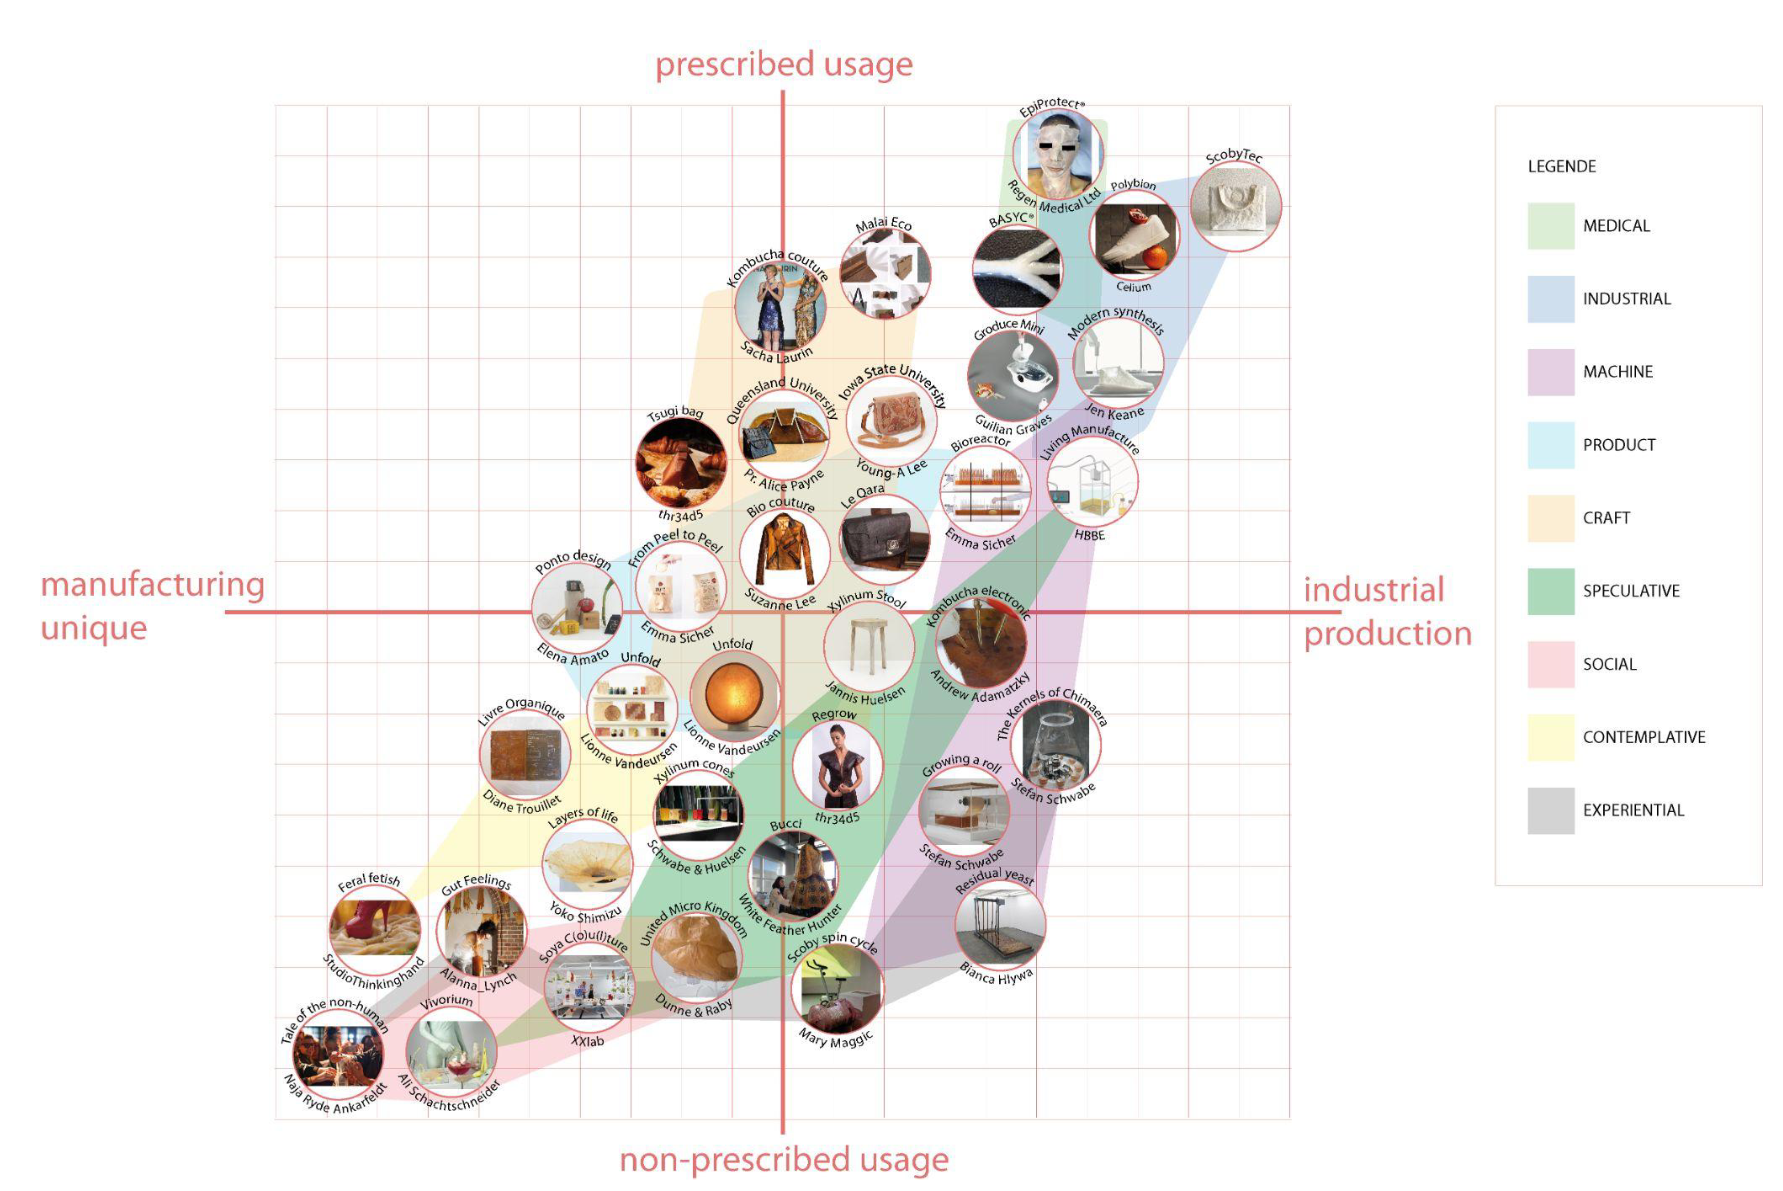
\includegraphics[width=1.4\textwidth]{images/mapping-practices-kombu.png} % Adjust width 
    \caption{Processes, Fabrication and Design with Kombucha Bacterial Cellulose: Mapping Practices from\cite{roussel2023processes}}
    \label{fig:graph-vivien}
\end{figure}




The work of zang et al\cite{zang2015investigation} describes how Bacterial cellulose (BC) exhibits exceptional biocompatibility, making it a promising material for various biomedical applications, particularly in vascular tissue engineering. Several studies have demonstrated that BC does not induce significant clotting or hemolysis when in contact with blood, indicating its favorable interactions with the bloodstream. This property is critical for any material intended for use in vascular implants or scaffolds, as it reduces the risk of thrombosis and ensures that blood flow is maintained without complications.
One of the earliest and most significant direct applications of bacterial cellulose (BC) membranes in the biomedical field is their use in wound dressings. 

Fontana et al. (1990)\cite{fontana1990acetobacter} were among the first to describe the use of BC as a substitute for burned skin. Since their pioneering work, the literature has seen a growing number of studies focused on wound dressing applications. Cellulose-based dressings are now widely recommended as a temporary solution for treating various types of wounds.\cite{de2016multipurpose} 
The cultivation techniques seem to be very classic in the future of microorganism cultivation. with classic laboratory equipment. however, in the recipes, the use of tea is hardly or not at all mentioned “The strain being used is a wild type microorganism isolated from a
decomposing homemade Matricaria sp. infusion”\cite{fontana1990acetobacter}. the quantities produced are deliberately small. but also the peridoe of growth is very reduced. 

\begin{marginfigure}
    \centering
    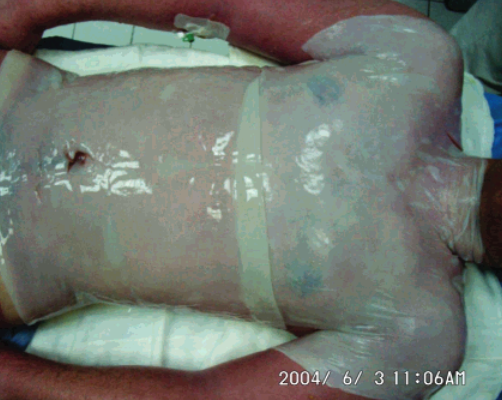
\includegraphics{images/medical_appl.png}    
    \caption{illustation BC use in medical applications from \cite{czaja2007future}}
    \label{fig:medical applications}
\end{marginfigure}

otherwise, from a more aesthetic point of view, jen keane's work on “this is grow".Materials designer and creative researcher Jen Keane developed her project “This is Grown” during her Master’s degree at Central Saint Martins, driven by her frustration with plastics.Blending design, science, technology, and craft, Keane is inspired by sustainability and intrigued by new digital and biological tools. In this project, she created a shoe upper grown as a single piece, using continuous yarn held together by cellulose produced by Komagataeibacter rhaeticus bacteria. This innovative, organism-driven approach enabled her to manipulate the growth process for a technique called "microbial weaving." 
The resulting hybrid material leverages the natural properties of bacterial cellulose, producing a strong, lightweight product with minimal waste. By employing a traditional weaving-like method where the warp is woven by Keane and the bacteria grow the weft at the nanoscale, the technique allows for intricate patterns and enhanced material strength in multiple directions.

In a similar vein to Jen Keane's work, Suzanne Lee, also associated with Central Saint Martins, pioneered the concept of BioCouture—a movement exploring DIY and traditional techniques for growing materials. Lee’s work has served as a foundational "nursery" of ideas for biodesign, integrating biology into fashion. By cultivating Komagataeibacter bacteria in a nutrient-rich solution, Lee was able to produce bacterial cellulose sheets that could be treated and crafted into wearable garments.

\begin{marginfigure}
    \centering
    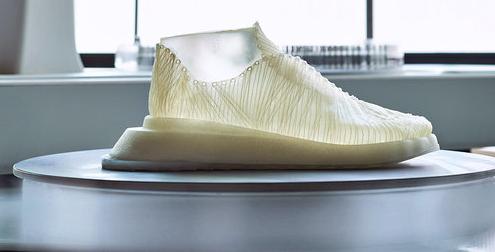
\includegraphics{images/jen_keane.png}
    \caption{Jen Keane - this is grow}
    \label{fig:jen_keane}
\end{marginfigure}

\begin{marginfigure}
    \centering
    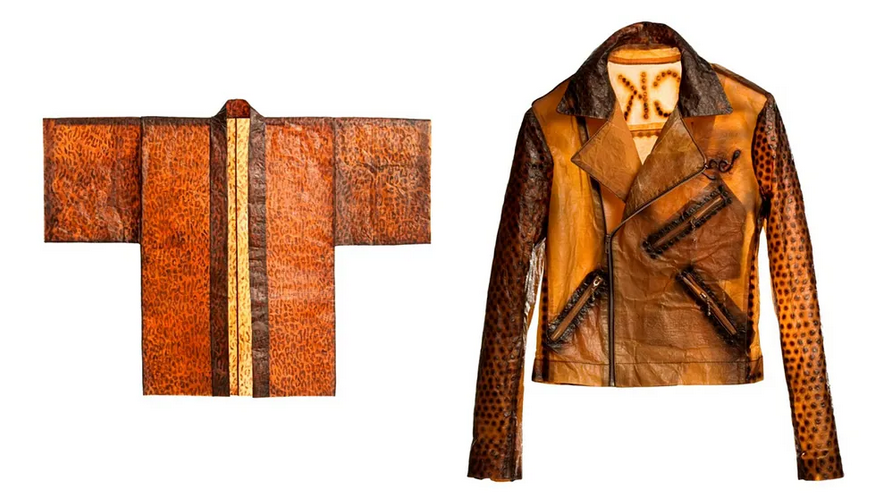
\includegraphics{images/suzanne_lee.png}
    \caption{Suzanne Lee - BioCouture}
    \label{fig:Suzanne Lee}
\end{marginfigure}

%\cite{caro2021bacterial}   maybe ???

Nicolae et Al. propose an framework \cite{nicolae2023biohybrid} of how build biohybride devince that incorporates electronics. 
Furthermore, they discuss the development of biohybride devine in HCI. The framework describe how prototyping with Bacterial cellulose. It distint three phase of BC life cycle where prototyping : Growth, Stabilization and Inanimate. 
The growth phase is mostly the part where add embed electronics or other particular material like textile. (This thesis will later discuss how the bioreactor can influence the material itself on this phase.)
The Stabilization phase is just after the growth phase before the biomaterial is dry. This phase enable 3D forming as the material is more maleable then after dry process. This phase was the phase use in medical applications for wound dressing, as the bacterial cellulose is still wet. the project this is grow by Jen keane might be between this two first phase.
The inanimate phase corresponds to the more traditional phase, after dry, where biomaterials resemble textile leather, and it's this part that Suzanne Lee focuses on in her biocouture project. 

\begin{figure}[h]
    \centering
    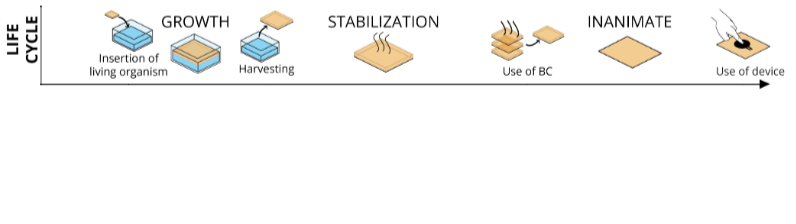
\includegraphics[width=1.4\textwidth]{images/phase-proto.png}
    \caption{BC life cycle phases as material from\cite{nicolae2023biohybrid}}
    \label{fig:life cycle}
\end{figure}




\subsection{Mycelium material}

\begin{marginfigure}
    \centering
    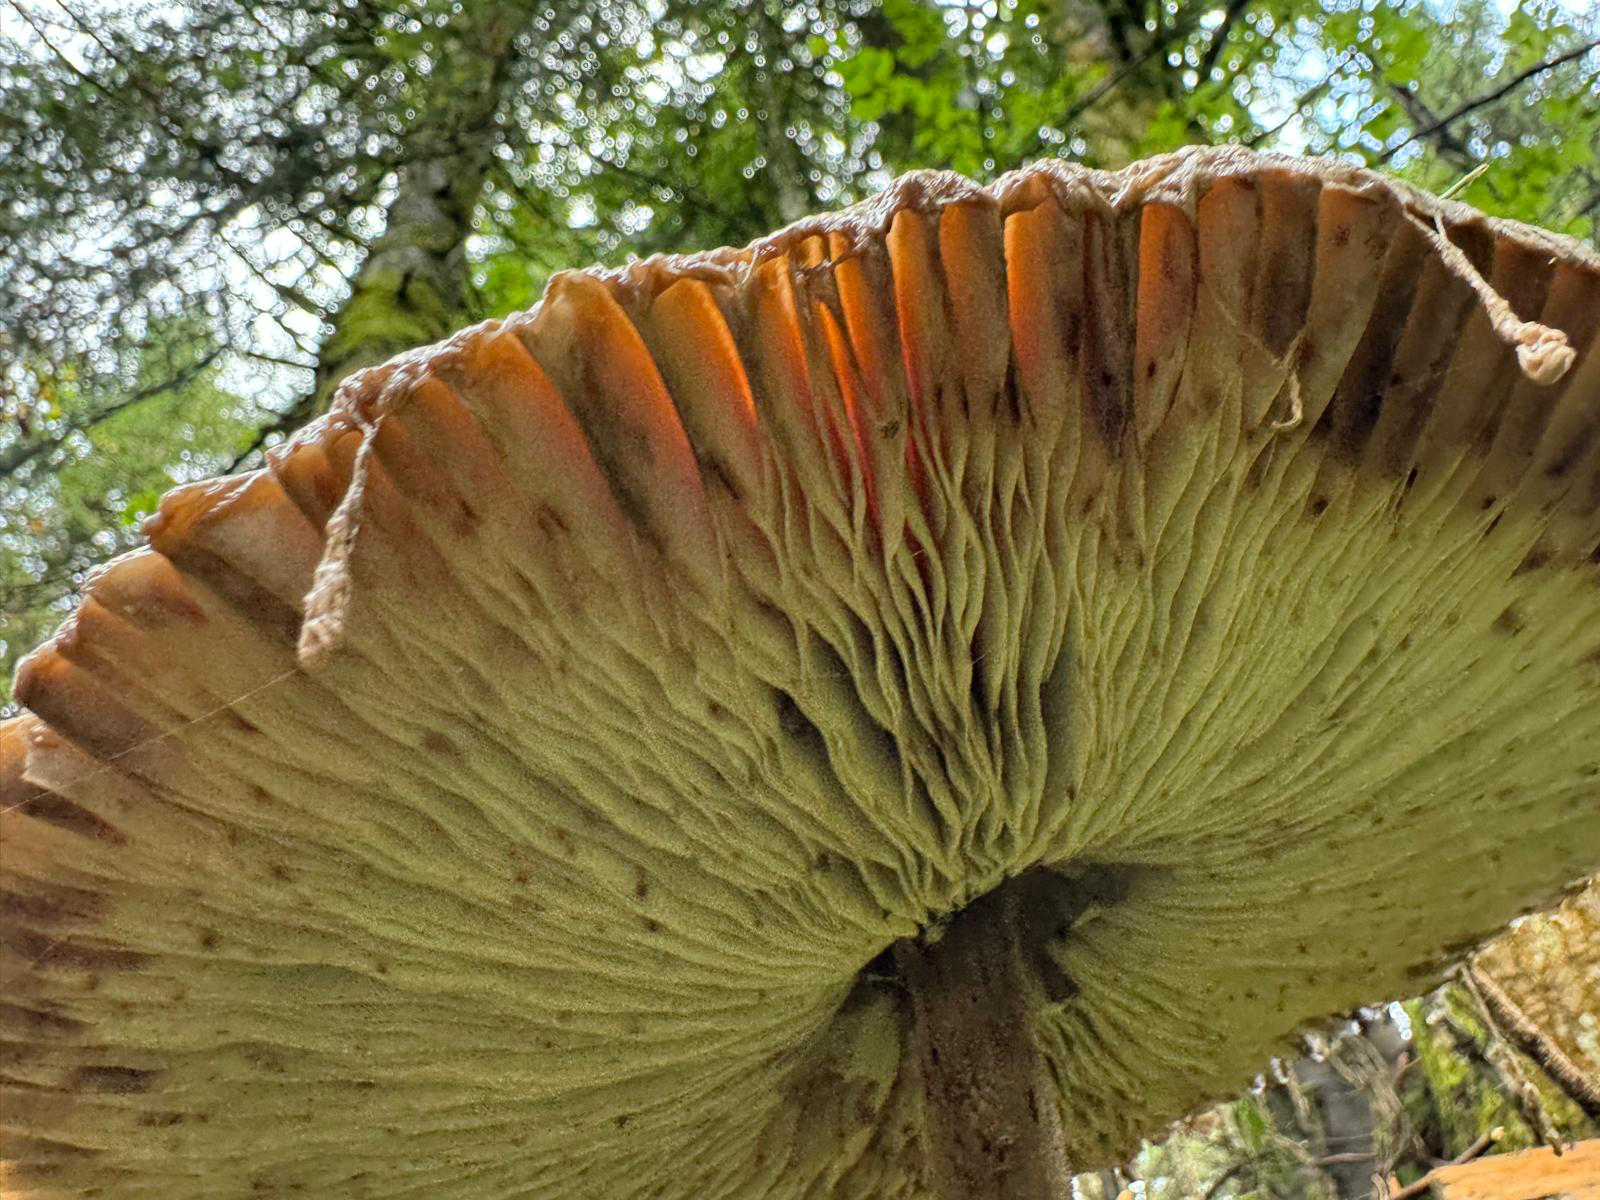
\includegraphics{images/champi.png}    
    \caption{pictured by me in Grenoble forest}
    \label{fig:champi}
\end{marginfigure}


\paragraph[short]{Definition}
"Mycelium is a root-like structure of a fungus consisting of a mass of branching, thread-like [called] hyphae."\cite{wikipediaMycelium}. Actually, The visible part of a mushroom during a forest walk is merely its surface structure. In the common sense, " mushroom " only refers to the fruiting bodie part,the reproductive part. 
On the other hand, Mycelium material, Mycomaterial, or mycelium-based biocomsites etc. Is a biofabricated material like bacterial cellulose. the general principle is to mix mycelium with an organic substrate. as in nature, the mycelium will secrete enzymes that dissolve its food, but also bond\cite{MonikaBrandićLipińskaHBBE} (\ref{fig:myco-bond}) and aglomarate the substate at cellular scale. 
Thus, we can give a shape to the inoculated substate and after the mycelium grow in all the substate like cellulose, it will be dry to give biocomposite. During these processes the substrate can be molded into various shapes to change the form of the biocomposite. 

\begin{figure}[h]
    \centering
    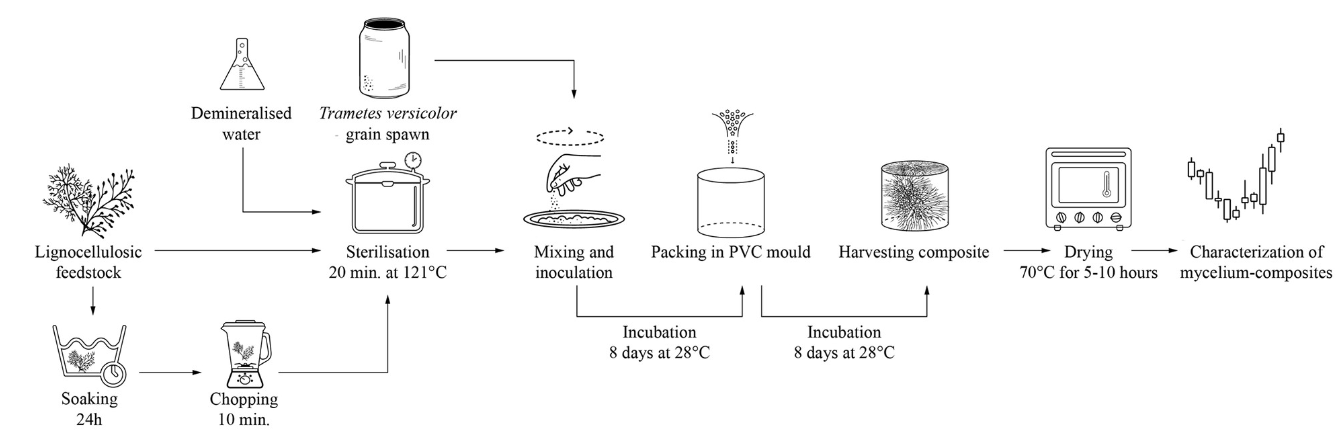
\includegraphics{images/Fabrication_process.png}
    \caption{Fabrication process of mycelium-based composites from  \cite{elsacker2019mechanical}}
    \label{fig:Fab_process}
\end{figure} 

\begin{marginfigure}
    \centering
    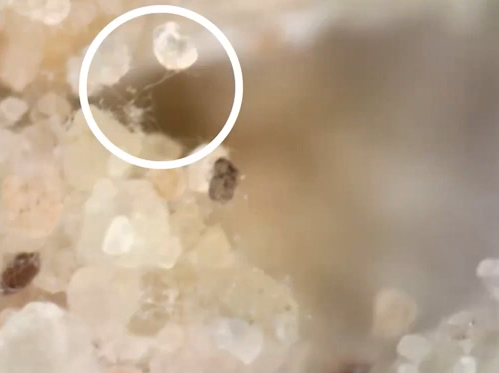
\includegraphics{images/bond-mycelium.png}    
    \caption{Mycelium at micro level on biocomposite from  Monika Brandić Lipińska | Space to Grow - Design of Biological Construction of Living Habitation on Mars}
    \label{fig:myco-bond}
\end{marginfigure}

A review of 2023,\cite{alaneme2023mycelium} show that Mycelium based composites, show that \ref{trend} the publication grew in the field.
This review also illustrates witch muchroom mycelium is use to build mycelium-base biocomposite, not all mushroom mycelia have the same characteristics, and some will produce harder or softer materials. on the other hand, the choice of substrate and the mass in which it is inoculated will also have an impact on the mechanical characteristics. furthermore, as the choice of mycelium itself influences how the mycelium will grow in the substrate, (a mycelium more adapted to a substrate with wood lignin for example will grow better in a substrate with wood lignin) some substrates give better results depending on the species of mushroom. 
however, it would seem that it is above all the choice of substrate that influences the mechanical properties, independently of the mycelium chosen.  

\begin{marginfigure}
    \centering
    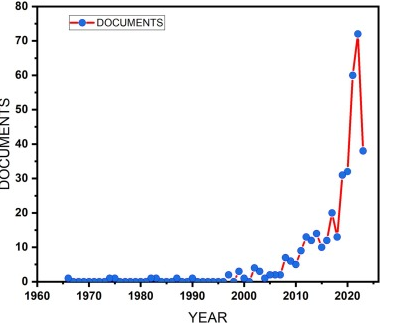
\includegraphics{images/publication on mycelium-based.png}    
    \caption{Trend of scientific publication on mycelium-based composites from 1966 to 2023 from \cite{alaneme2023mycelium}}
    \label{fig:trend}
\end{marginfigure}

Research by Elsacker et al.\cite{elsacker2019mechanical} and Yang et al.\cite{yang2017physical} demonstrates that the design of the substrate mold significantly influences the mechanical properties—such as compressive strength, stiffness, and Young’s modulus—of mycelium-based composites (MBCs). Mold shape, density, and stiffness play a crucial role as the inoculated mix of mycelium and substrate fills the mold, impacting the final density and fiber orientation of the MBCs. Various packing methods, including polyethylene and porous bags, PVC, and thermo-formed plastic molds, are employed, with each method affecting the quality and structure of the fungal skin. Optimal mold design remains a key area for further research to improve MBC production.

Reports indicate that the low thermal conductivity, high acoustic absorption, and fire-resistant qualities of MBCs have made them highly suitable for use in building and construction. \cite{ghazvinian2019mycelium}

\paragraph{Use}

There is no mapping practice of mycelium in the litterature like Roussel et al.'s \cite{roussel2023processes} did for SCOBY. but we believe that the mycelium shares similarities with the interdisciplinary clustering parameters presented.
Mycelium-based biocomsites have been uses both in the speculative and industrial sectors as well as in research.

\begin{figure}[h]
    \centering
    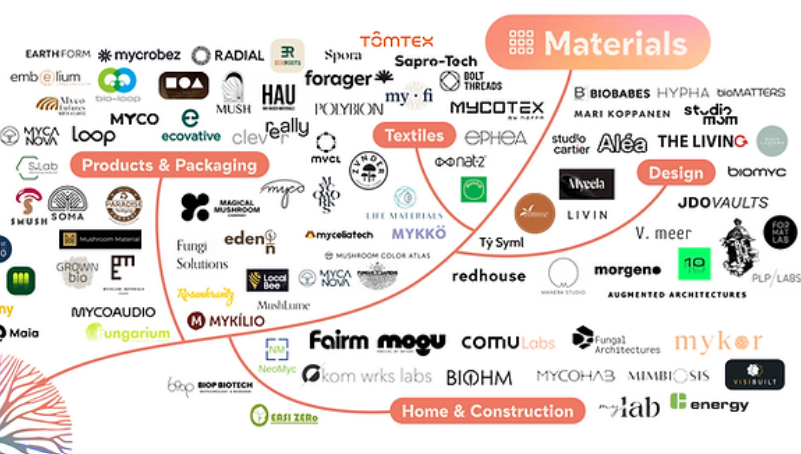
\includegraphics{images/mycelium-indus-tree.png}
    \caption{materials field industry for Mycelium composite}
    \label{fig:indus-tree}
\end{figure}

The mapping of Mycostory, illustrates (a bit) different scector in Mycelium materials industry. design practice aside, there are 3 main ways in which MBC tends to be used functionally: packaging, construction, and textiles. 
it's mainly packaging and construction that are similar to biocomposite techniques. the textile sector is full of other methods for making mycelium leather that differ from mycelium-based composites. 



Ecovative is a pioneer in this field, particularly in packaging, where their products demonstrate how mycelium-based composites (MBCs) can replace traditional, environmentally harmful materials like Styrofoam. By using agricultural waste combined with mycelium, Ecovative creates biodegradable packaging that performs similarly to synthetic foams, offering both protective qualities and a fully compostable lifecycle. they've managed to scale up the techniques we've developed before so that they can supply other companies with products in large quantities. 
\begin{figure}[h]
    \centering
    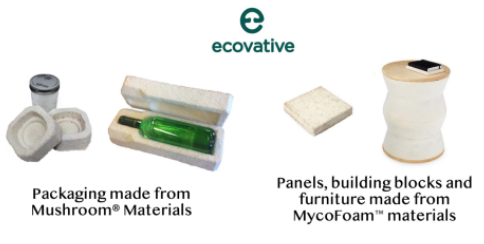
\includegraphics{images/ecovative.png}
    \caption{}
    \label{fig:ecovative}
\end{figure} 

The works of Monika Brandić Lipińska and NIAC (NASA innovative advanced concept) suggests the use of mycelium\cite{rothschild2019myco} to build on mars mycelium structures\cite{brandic2022biological}.

The works of Monika Brandić Lipińska and NASA’s Innovative Advanced Concepts (NIAC) propose utilizing mycelium as a sustainable and adaptable material for constructing habitats on Mars. Rothschild et al. (2019) \cite{rothschild2019myco} in their NIAC report suggest that mycelium-based structures could be grown on-site using local Martian resources, reducing the logistical challenges and costs associated with transporting building materials from Earth’s adaptability and self-repair potential, combined with its low resource requirements, make it a promising candidate for developing structures in the harsh Martian environment.

Brandić Lipińska’s research\cite{brandic2022biological} further explores how biological materials like mycelium could be integrated into extraterrestrial construction. Her work emphasizes the environmental and structural benefits of mycelium, such as thermal insulation, radiation shielding, and the potential to grow complex architectures with minimal human intervention. By incorporating mycelium into Martian habitat designs, these studies pave the way for innovative construction techniques that leverage living organisms to create adaptable, eco-friendly, and self-sustaining habitats in space .

From a terrestrial perspective, Mogu\cite{MoguMogu} is at the forefront of manufacturing mycelium-based composites (MBC) specifically tailored for applications in building insulation. Mogu’s approach capitalizes on the intrinsic properties of mycelium to create materials that offer high thermal resistance and effective sound absorption

There are numerous projects demonstrating the benefits of biocomposite mycelium in architecture. Like HBBE's Bioknit, the living New york by Hy-fy, or the growing pavilion\cite{thegrowingpavilion}. either from a structural point of view, or through the manufacture of panels.  

\begin{marginfigure}
    \centering
    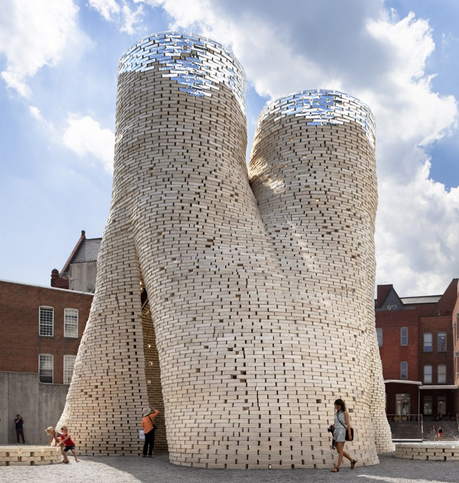
\includegraphics{images/ThelivingNewYork_Hy-Fi.png}    
    \caption{}
    \label{fig:NY}
\end{marginfigure}

\begin{marginfigure}
    \centering
    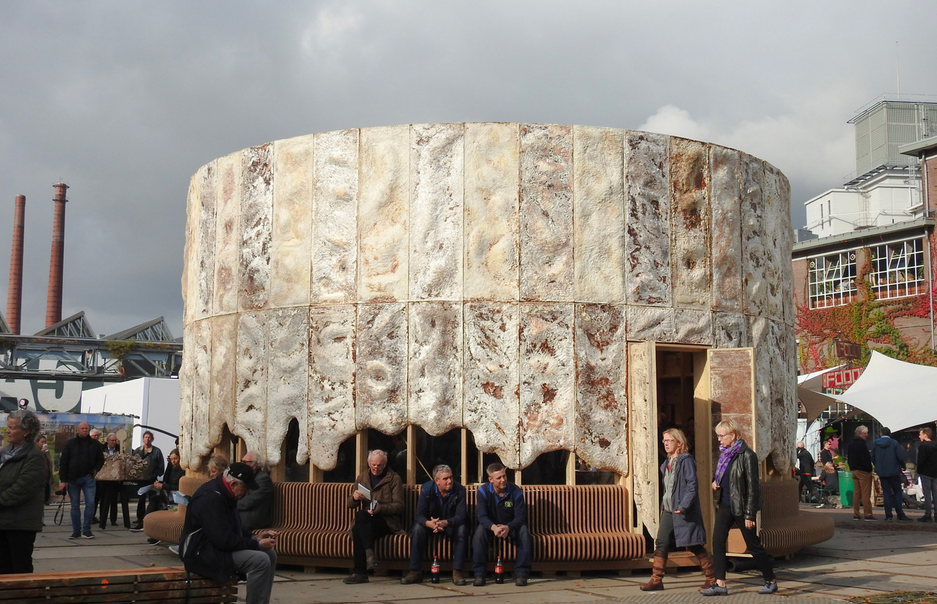
\includegraphics{images/TGP.png}    
    \caption{}
    \label{fig:the living}
\end{marginfigure}

\begin{marginfigure}
    \centering
    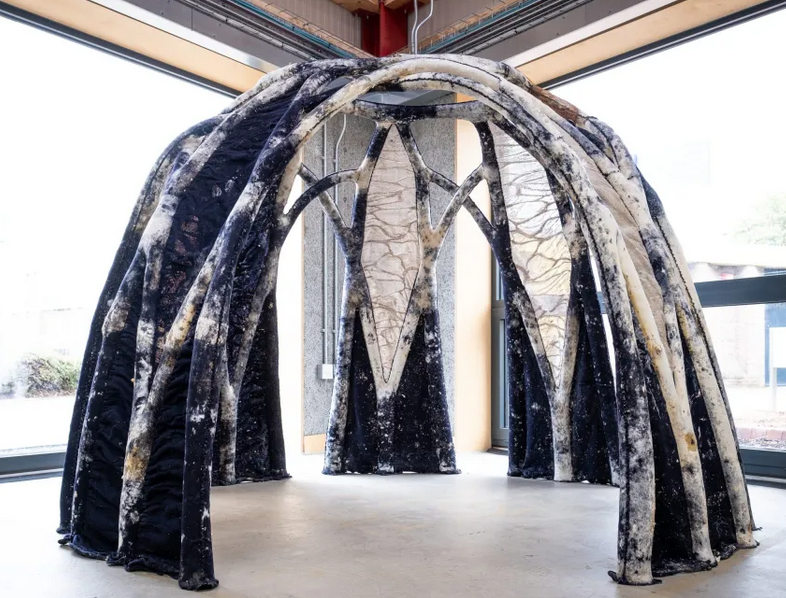
\includegraphics{images/Hbbe_bioknit.png}    
    \caption{}
    \label{fig:mycohbbe}
\end{marginfigure}



\subsection{Other Biomaterial}

There are, of course, other types of biomaterials that can be put forward as sustainable alternatives to plastics and other petroleum-based products. 
These may differ in their production methods, unlike mycelium or scoby, which are co-products of living organisms. These other materials are not necessarily produced by living organisms. 

There's the study on gelatin alginate-based bioplastics, which are manufactured using conventional chemical processes. 
There are other forms of organic leather from coconut, banana and pineapple.

Eric Klarenbeek and Maartje Dros have developed an innovative bioplastic derived from algae\cite{algaelab}, aiming to replace fossil-based plastics with renewable materials. Collaborating with Atelier Luma, they grow, dry, and process algae into a 3D-printable polymer suitable for producing a wide range of products, from containers to furniture.

The Silk Pavilion, from Neri Oxman , explored the blend of digital and biological construction. Inspired by the natural 3D cocoon-spinning process of silkworms, a robotic arm laid the groundwork for a three-meter dome, which 6,500 silkworms then completed by spinning silk sheets instead of cocoons

\begin{marginfigure}
    \centering
    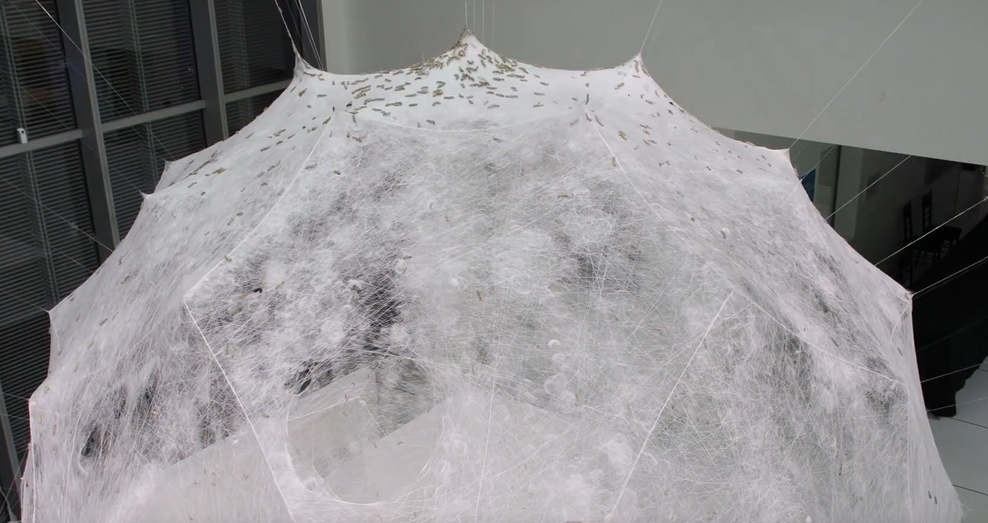
\includegraphics{images/Silk_Pavilion.png}    
    \caption{Silk Pavilion I from Neri Oxman}
    \label{fig:oxman}
\end{marginfigure}

\begin{marginfigure}
    \centering
    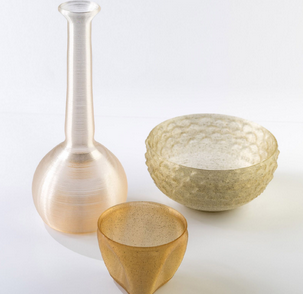
\includegraphics{images/ALGAE.png}    
    \caption{Bioplastic derived from algae by \cite{algaelab}}
    \label{fig:algae}
\end{marginfigure}

Some of them don't really use machines like bioreactors for their production.  
That's how scoby and mycelium are related. that's why they're presented here as 2 different biomateraixes, but they share similar methods for optimizing their production, and for creating new material functions/forms with the help of bioreactors. 



\section{Bioreactor \& Controlled Environment }



We have deliberately omitted, or at least very rarely mentioned, the use of machines to manufacture biomaterials. In order to focus on the material itself 
 
However, machines have a fundamental role to play in production, in optimizing growth and in changing growth conditions, which adds new characteristics to the material in situ.  
They also bring standardization to material production, and enable a more rigorous methodology for understanding biomaterial growth.
At the same time, they allow real-time monitoring, collection and modification of climatic growth conditions. Data that is extremely useful for understanding and optimizing the process.

Bioreactor, Controlled Environment Systems, Incubator or Fermentator, refers to more or less the same general concept, they differ mainly in expressing which living organism is involved with which method. for example, the term bioreactor is more commonly used in the case of bacteria and the early stages of mushroom development, while the term controlled environment is more commonly used in the case of agriculture.
So generally speaking, these systems are :

\- -- An Isolated spaces to limit interaction with external conditions.

\- -- A bench of Sensor twinned with one or more actuators. Actuator that can take the form of fans, peristaltic pumps, foggers, lights, in other words anything that can directly or indirectly change the growth environment and climatic conditions (change in temperature, addition of nutrients, etc.) 

\- -- A microcontroller that reads sensor values and decides whether to activate actuators, and optionally saves or sends data for analysis or monitoring. 

In addition to all this, the second great advantage of these machines is their ability to interfere with the growing process to add new functionalities. in other words, to constrain, to add other materials to the growing process, to force living organisms to adopt unnatural growing behaviors. for example, cellulose grows directly in the shape of a handbag, or by adding meshes of textile threads to the cellulose, like jen leane.   
Or to manage oxygen concentrations to force unnatural overproduction of mushroom caps texture.

\subsection{Bioreactor S.C.O.B.Y}

Several bioreactor projects have been used for different purposes. some are more specialized in optimizing cellulose production, others in changing the form of the cellulose, or simply to control the climatic parameters of growth. 

Although there is no very precise study on this subject, the optimum environmental conditions for cellulose growth would be to have a good source of carbon in the medium \cite{ruka2012altering} (sugars), a temperature between 22°C and 30°C, and sterilization of the culture medium in an autoclave or at least cleaning with alcohol. 

Hornung's thesis\cite{hornung2010optimising} work identified ways of optimizing growth in relation to the “self-asphyxiation” problem, as cellulose grows up and down from the surface of the liquid, with nutrients in the culture medium and oxygen in the air above.
Based on this observation, the Hornung bioreactor releases nutrients and oxygen directly from above in the form of aerosseol. 
Which has greatly increased cellulose production. 

\begin{figure}[h]
    \centering
    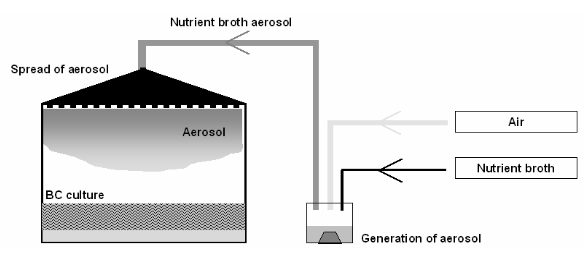
\includegraphics{images/aerosol.png}
    \caption{Hornung aerosol bioreactor from \cite{hornung2010optimising}}
    \label{fig:aerosol}
\end{figure} 

The work of Soleimani, Ali, et al.rotary bioreactor aim to grow bacterial cellulose in 3D by inplementin rotating disc in the culture medium. 

The research by Soleimani et al.\cite{soleimani2021design} designed a bench-scale rotating biological contactor (RBC) to optimize bacterial cellulose production. Key variables, such as disk rotation speed, spacing, type, and aeration, were examined. The highest BC yield was achieved using integrated polyethylene discs rotating at 13 rpm, spaced 1 cm apart, with a 16-disk configuration. Aeration, introduced via an aquarium pump, further increased BC yield, with wet and dry weights rising by over 64\% and 47\%, respectively, compared to non-aerated RBC. Compared to static culture, aerated RBC fermentation achieved over 90.7\% higher wet weight and 71\% higher dry weight, confirmed by SEM analysis at the nanoscale.
The studies also show that bacterial cellulose can grow in 3D by inplementin rotating disc in the culture medium.
This is why the studies also show a increased of production of BC is because increase the surface of interaction with air, increase the production of BC and crete 3D structure of BC.

The projet of Roussel combines the techniques described earlier by jen keane and rotary bioreactors. the project consisted in making 3D cellulose which would not grow directly on the surface of the liquid but on a chosen shape which, like Soleimani's discs, would emerge on the surface of the liquid in rotation. 
The shape was printed in 3D and a textile mesh on the shape allowed the cellulose to adhere well to the shape. 
This technique allows the efficient production of cellulose in 3D, which means that the bioreactor changes the natural conditions of growth and produces a greater quantity of cellulose. 

\begin{figure}[h]
    \centering
    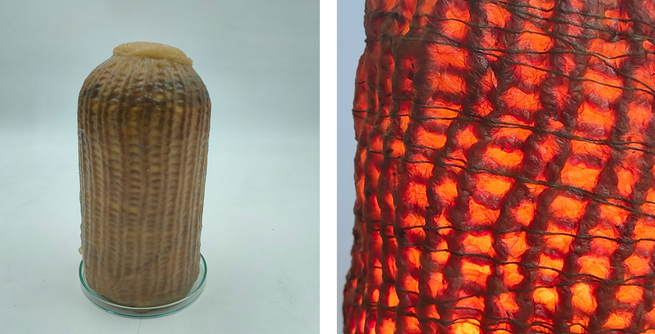
\includegraphics{images/machinevivien.png}
    \caption{resuslt of combine technics by Roussel}
    \label{fig:3Droussel}
\end{figure} 

Hub for biotechnology in the built environment (HBBE) develop a new kind of bioreactor mix with a 3D priter. This project seeks to develop a 3D printing process that leverages bacterial cellulose (BC) synthesis, using live microbes to produce 3D functionally graded materials. It integrates genetically engineered microbes and a specialized bioreactor within a new kind of 3D printer, aiming to establish principles for industrial-scale biological fabrication. The potential applications of this biofabrication system range from biomedical materials to complex composites.
Hardware: Two prototypes are under development:  a bioreactor with BC-producing bacteria and optogenetic E. coli that produces color in response to light, and a bioreactor with BC-producing bacteria, using enzymes to selectively weaken cellulose in specific areas. The modular system, built from an EvoBot-based design, includes a rail-mounted chemical dripper and a pellicle height monitor.
Wetware: This part of the project aims to optimize BC pellicle growth. Using an automatic nutrient delivery system to maintain the BC at the air-liquid interface, continuous, homogeneous BC layers over 8 cm thick have been achieved. A patent application is underway for this method.




%other ? 






\subsection{ Controlled
Environment Mycelium}

Controlled Environment Mycelium based biocomposite quite similar to the imcubators used to grow mushrooms for nourirtutre. The difference lies mainly in the substrates used, the climatic conditions and the use of molds.

The classic controlled environment, like the martha tent \ref{marthatent} 
from fungi academy consists of a grow tent, a fogger, an air outlet to avoid asphyxiating the mycelium and promoting contaminants, light depending on the species, and termic resistances to control teperature.  

\begin{figure}[h]
    \centering
    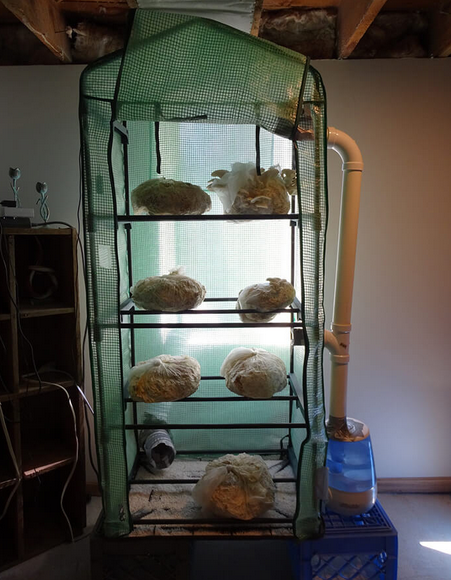
\includegraphics{images/classicalmyceliumtent.png}
    \caption{classic controlled environment, martha tent \ref{marthatent} }
    \label{fig:marthatent}
\end{figure} 

On a large scale ecovative has developed huge chambers for growing biocompisites \cite{ecovativepatent}. everything is automated and the data is even used for machine learning algorithms to optimize production. 
In this growth chamber ecovative has also developed a complex method for air contact, so that the mycelium is in the best possible contact with the oxygen. 

Lovely Trash Column project from blast studio have a differenct approach\cite{blaststudio}. They directly included mycelium in a substate which will then be put into a custom 3d printer to print the substrate. 
In order to directly impregnate forms that will give MBCs after mycelium growth. 

\begin{figure}[h]
    \centering
    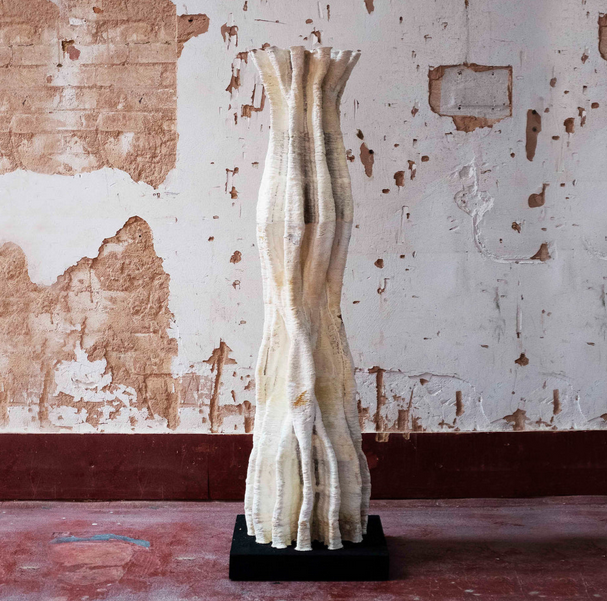
\includegraphics{images/printMycelium.png}
    \caption{image from \cite{blaststudio}}
    \label{fig:blasttrash}
\end{figure} 

\begin{marginfigure}
    \centering
    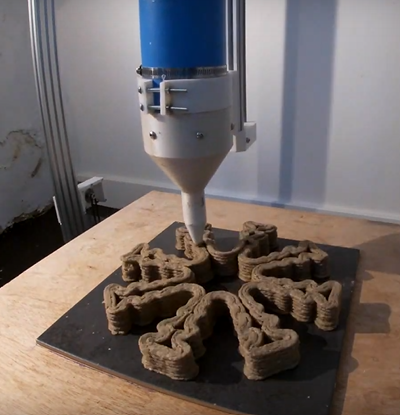
\includegraphics{images/printMycelium2.png}
    \caption{image from \cite{blaststudio}}
    \label{fig:blasttrash}
\end{marginfigure} 


From a low-tech point of view, some systems directly integrate posse not in machines but directly in the spaces of the quaditien that integrate the good climatic condition. 

The biosphere experience project, which takes place in what a parisian apartment might be like in 2040, involves a multitude of low-tech projects to feed, heat, eat and wash oneself for 4 months. The project incorporates mycelium loaves in their showers to provide the necessary conditions for mycelium growth. 


\begin{figure}[h]
    \centering
    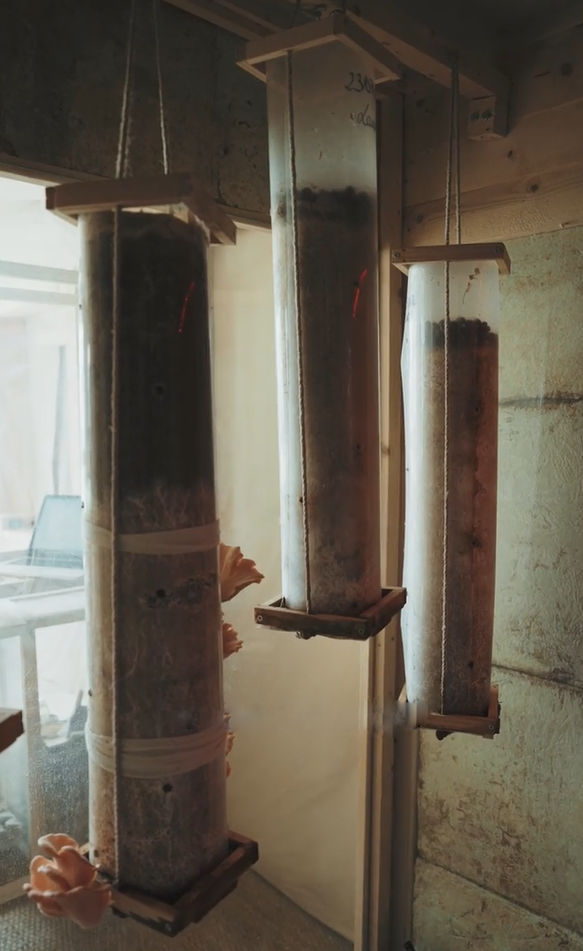
\includegraphics{images/lowtechdouche2.png}
    \caption{image from \cite{lowtechmyco}}
    \label{fig:blasttrash}
\end{figure} 


\section{Discution and limitation}